% Options for packages loaded elsewhere
\PassOptionsToPackage{unicode}{hyperref}
\PassOptionsToPackage{hyphens}{url}
%
\documentclass[
]{article}
\usepackage{amsmath,amssymb}
\usepackage{lmodern}
\usepackage{iftex}
\ifPDFTeX
  \usepackage[T1]{fontenc}
  \usepackage[utf8]{inputenc}
  \usepackage{textcomp} % provide euro and other symbols
\else % if luatex or xetex
  \usepackage{unicode-math}
  \defaultfontfeatures{Scale=MatchLowercase}
  \defaultfontfeatures[\rmfamily]{Ligatures=TeX,Scale=1}
\fi
% Use upquote if available, for straight quotes in verbatim environments
\IfFileExists{upquote.sty}{\usepackage{upquote}}{}
\IfFileExists{microtype.sty}{% use microtype if available
  \usepackage[]{microtype}
  \UseMicrotypeSet[protrusion]{basicmath} % disable protrusion for tt fonts
}{}
\makeatletter
\@ifundefined{KOMAClassName}{% if non-KOMA class
  \IfFileExists{parskip.sty}{%
    \usepackage{parskip}
  }{% else
    \setlength{\parindent}{0pt}
    \setlength{\parskip}{6pt plus 2pt minus 1pt}}
}{% if KOMA class
  \KOMAoptions{parskip=half}}
\makeatother
\usepackage{xcolor}
\usepackage[margin=1in]{geometry}
\usepackage{color}
\usepackage{fancyvrb}
\newcommand{\VerbBar}{|}
\newcommand{\VERB}{\Verb[commandchars=\\\{\}]}
\DefineVerbatimEnvironment{Highlighting}{Verbatim}{commandchars=\\\{\}}
% Add ',fontsize=\small' for more characters per line
\usepackage{framed}
\definecolor{shadecolor}{RGB}{248,248,248}
\newenvironment{Shaded}{\begin{snugshade}}{\end{snugshade}}
\newcommand{\AlertTok}[1]{\textcolor[rgb]{0.94,0.16,0.16}{#1}}
\newcommand{\AnnotationTok}[1]{\textcolor[rgb]{0.56,0.35,0.01}{\textbf{\textit{#1}}}}
\newcommand{\AttributeTok}[1]{\textcolor[rgb]{0.77,0.63,0.00}{#1}}
\newcommand{\BaseNTok}[1]{\textcolor[rgb]{0.00,0.00,0.81}{#1}}
\newcommand{\BuiltInTok}[1]{#1}
\newcommand{\CharTok}[1]{\textcolor[rgb]{0.31,0.60,0.02}{#1}}
\newcommand{\CommentTok}[1]{\textcolor[rgb]{0.56,0.35,0.01}{\textit{#1}}}
\newcommand{\CommentVarTok}[1]{\textcolor[rgb]{0.56,0.35,0.01}{\textbf{\textit{#1}}}}
\newcommand{\ConstantTok}[1]{\textcolor[rgb]{0.00,0.00,0.00}{#1}}
\newcommand{\ControlFlowTok}[1]{\textcolor[rgb]{0.13,0.29,0.53}{\textbf{#1}}}
\newcommand{\DataTypeTok}[1]{\textcolor[rgb]{0.13,0.29,0.53}{#1}}
\newcommand{\DecValTok}[1]{\textcolor[rgb]{0.00,0.00,0.81}{#1}}
\newcommand{\DocumentationTok}[1]{\textcolor[rgb]{0.56,0.35,0.01}{\textbf{\textit{#1}}}}
\newcommand{\ErrorTok}[1]{\textcolor[rgb]{0.64,0.00,0.00}{\textbf{#1}}}
\newcommand{\ExtensionTok}[1]{#1}
\newcommand{\FloatTok}[1]{\textcolor[rgb]{0.00,0.00,0.81}{#1}}
\newcommand{\FunctionTok}[1]{\textcolor[rgb]{0.00,0.00,0.00}{#1}}
\newcommand{\ImportTok}[1]{#1}
\newcommand{\InformationTok}[1]{\textcolor[rgb]{0.56,0.35,0.01}{\textbf{\textit{#1}}}}
\newcommand{\KeywordTok}[1]{\textcolor[rgb]{0.13,0.29,0.53}{\textbf{#1}}}
\newcommand{\NormalTok}[1]{#1}
\newcommand{\OperatorTok}[1]{\textcolor[rgb]{0.81,0.36,0.00}{\textbf{#1}}}
\newcommand{\OtherTok}[1]{\textcolor[rgb]{0.56,0.35,0.01}{#1}}
\newcommand{\PreprocessorTok}[1]{\textcolor[rgb]{0.56,0.35,0.01}{\textit{#1}}}
\newcommand{\RegionMarkerTok}[1]{#1}
\newcommand{\SpecialCharTok}[1]{\textcolor[rgb]{0.00,0.00,0.00}{#1}}
\newcommand{\SpecialStringTok}[1]{\textcolor[rgb]{0.31,0.60,0.02}{#1}}
\newcommand{\StringTok}[1]{\textcolor[rgb]{0.31,0.60,0.02}{#1}}
\newcommand{\VariableTok}[1]{\textcolor[rgb]{0.00,0.00,0.00}{#1}}
\newcommand{\VerbatimStringTok}[1]{\textcolor[rgb]{0.31,0.60,0.02}{#1}}
\newcommand{\WarningTok}[1]{\textcolor[rgb]{0.56,0.35,0.01}{\textbf{\textit{#1}}}}
\usepackage{longtable,booktabs,array}
\usepackage{calc} % for calculating minipage widths
% Correct order of tables after \paragraph or \subparagraph
\usepackage{etoolbox}
\makeatletter
\patchcmd\longtable{\par}{\if@noskipsec\mbox{}\fi\par}{}{}
\makeatother
% Allow footnotes in longtable head/foot
\IfFileExists{footnotehyper.sty}{\usepackage{footnotehyper}}{\usepackage{footnote}}
\makesavenoteenv{longtable}
\usepackage{graphicx}
\makeatletter
\def\maxwidth{\ifdim\Gin@nat@width>\linewidth\linewidth\else\Gin@nat@width\fi}
\def\maxheight{\ifdim\Gin@nat@height>\textheight\textheight\else\Gin@nat@height\fi}
\makeatother
% Scale images if necessary, so that they will not overflow the page
% margins by default, and it is still possible to overwrite the defaults
% using explicit options in \includegraphics[width, height, ...]{}
\setkeys{Gin}{width=\maxwidth,height=\maxheight,keepaspectratio}
% Set default figure placement to htbp
\makeatletter
\def\fps@figure{htbp}
\makeatother
\setlength{\emergencystretch}{3em} % prevent overfull lines
\providecommand{\tightlist}{%
  \setlength{\itemsep}{0pt}\setlength{\parskip}{0pt}}
\setcounter{secnumdepth}{-\maxdimen} % remove section numbering
\ifLuaTeX
  \usepackage{selnolig}  % disable illegal ligatures
\fi
\IfFileExists{bookmark.sty}{\usepackage{bookmark}}{\usepackage{hyperref}}
\IfFileExists{xurl.sty}{\usepackage{xurl}}{} % add URL line breaks if available
\urlstyle{same} % disable monospaced font for URLs
\hypersetup{
  pdftitle={R Basics for Paleoecologists},
  pdfauthor={C.A. Kiahtipes},
  hidelinks,
  pdfcreator={LaTeX via pandoc}}

\title{R Basics for Paleoecologists}
\author{C.A. Kiahtipes}
\date{2/14/2023}

\begin{document}
\maketitle

\hypertarget{apd-workshop-series-r-basics-for-paleoecologists.}{%
\subsection{APD Workshop Series: R Basics for
Paleoecologists.}\label{apd-workshop-series-r-basics-for-paleoecologists.}}

\hfill\break

This is meant to be a simple guide to help otherwise busy
paleoecologists make use of some helpful tools for conducting research
and publishing. All the while, you will also be making your work
reproducible.\\
\strut \\
\strut \\

\hypertarget{required-software-and-download-instructions}{%
\subsubsection{Required Software and Download
Instructions}\label{required-software-and-download-instructions}}

\hfill\break

For this workshop we will be using two separate, but related pieces of
open-source software: R and R Studio.\\
\strut \\
R is a standalone open-source software for statistical analysis. It has
an interesting history (you can find more here), but it is \emph{both} a
programming language and an environment within which you can use the
language to execute commands. Thus, it is described as the ``R
Statistical Computing Environment''. R is an instantiation of a tiny
universe with many rules, few (or none!) of which you know.\\
\strut \\
R Studio is a wrapper for R that allows us to see a bit more of what is
going on inside of R and to control it through the window rather than
exclusively through the ``console''. R Studio knows the rules so you
don't have to. Much like a spell-checker in word processing, R Studio
checks your code for you. More on this later.\\
\strut \\
\strut \\

\hypertarget{installing-r-statistical-computing-environment}{%
\paragraph{Installing R Statistical Computing
Environment}\label{installing-r-statistical-computing-environment}}

\hfill\break

\textbf{First}, you need to install R from
\href{https://cran.r-project.org/}{cran.r-project.org}. Click this link
or the logo below, at the top of the page you will find a section titled
``Download and Install R'' and choose the appropriate download for your
operating system (OS).\\

\href{https://cran.r-project.org/}{\includegraphics[width=0.25\textwidth,height=\textheight]{https://www.r-project.org/logo/Rlogo.png}}

\hfill\break
It should look something like this:

\begin{figure}

{\centering 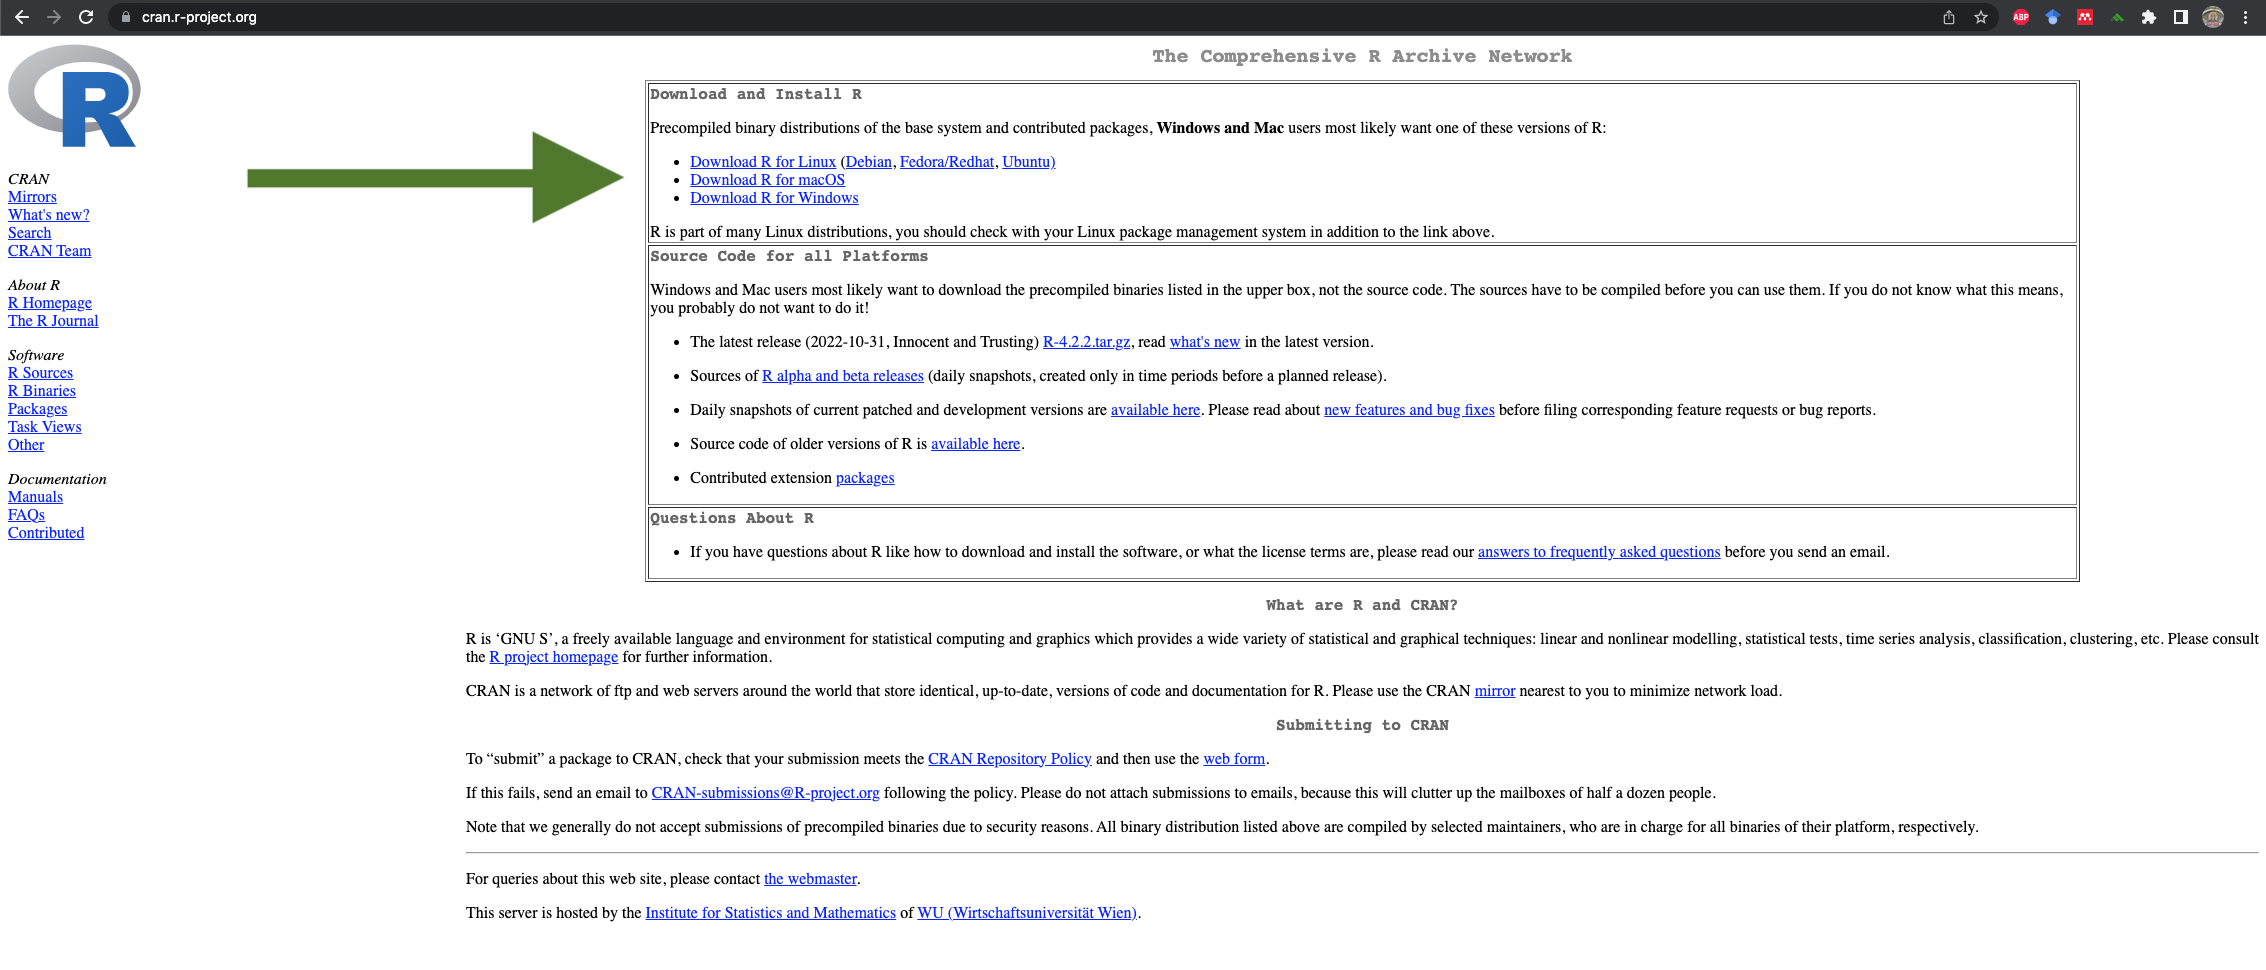
\includegraphics{images/cran_page} 

}

\caption{**Figure 1**. cran.R-project website landing page.}\label{fig:screenshot of R main site}
\end{figure}

\hfill\break

Once you've selected the R version for your OS, you'll be given some
download options. Select ``base'' and download the .exe file (Windows).

\begin{figure}

{\centering 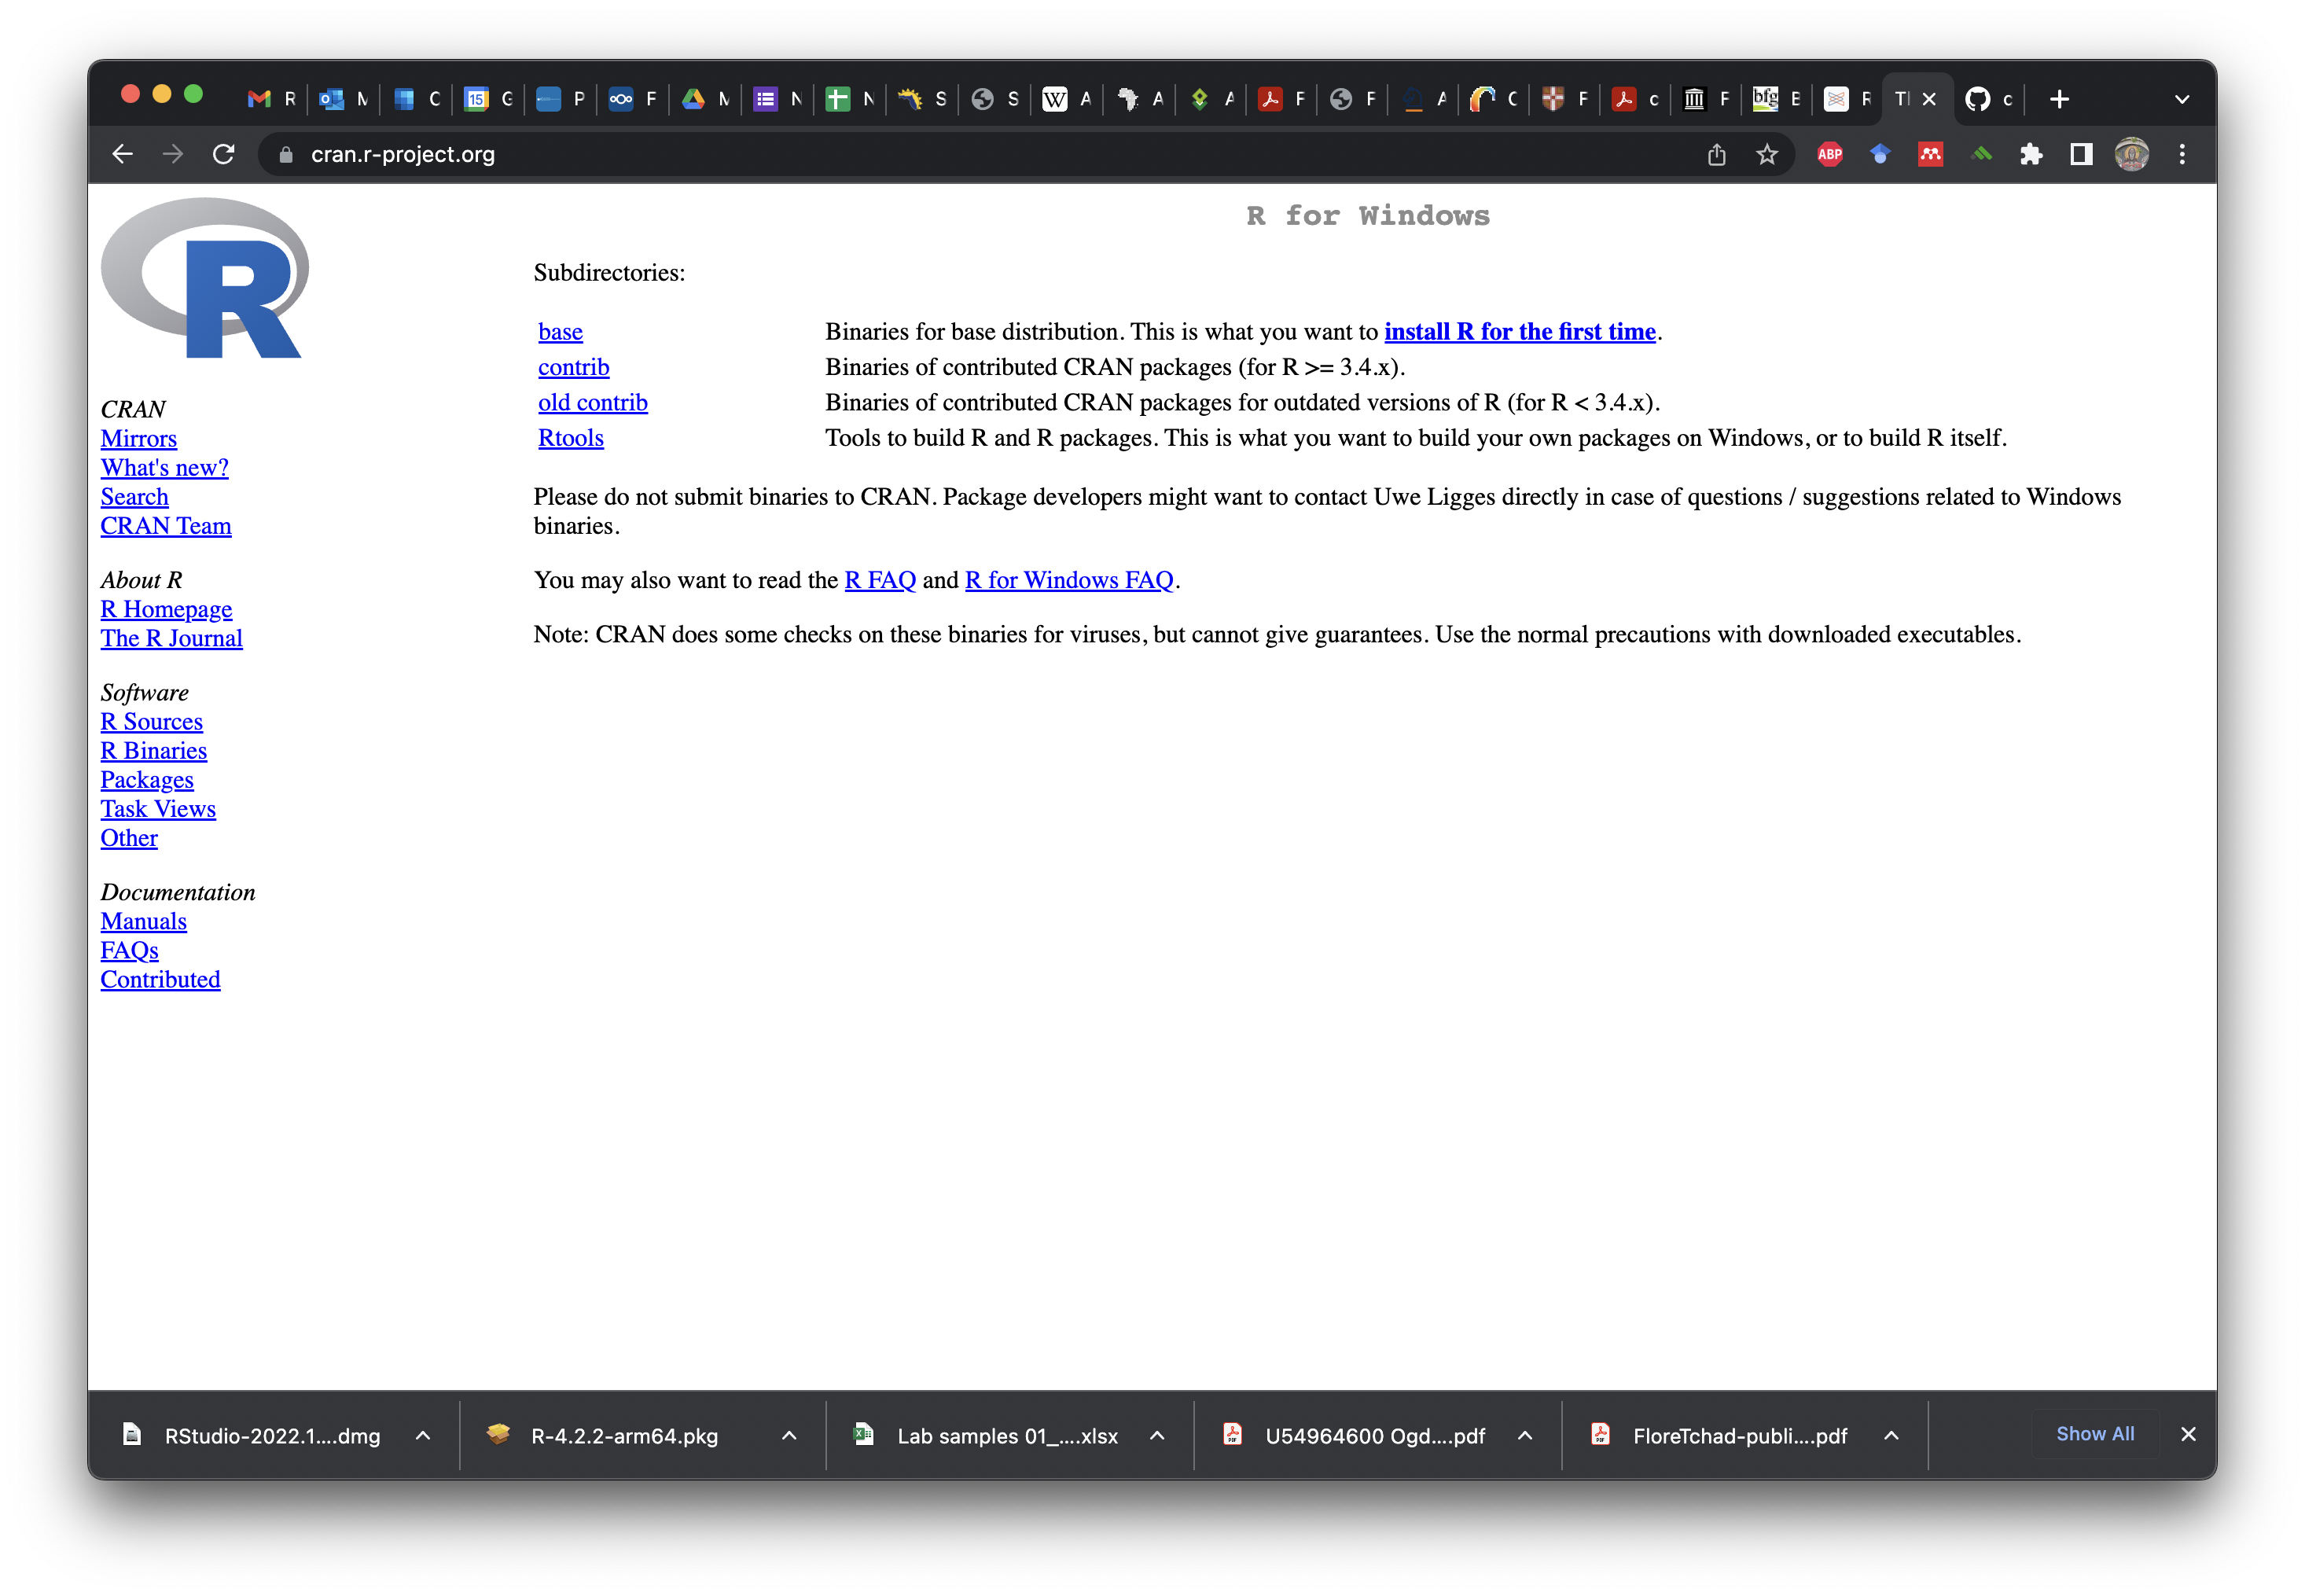
\includegraphics{images/cran_download} 

}

\caption{**Figure 2.** cran.R-project windows download options, select 'base'.}\label{fig:screenshot of download options}
\end{figure}

\hfill\break

Double-click on this file and follow the instructions from your
machine's prompts for installation. This differs slightly between each
operating system and the version of the operating system you're using.

If you're using macOS, you will be directed to a slightly different
looking page with multiple download options. Here, you much choose a
package based on the version of the macOS you're using. If you're using
OS 11 or greater (Apple names their updates, so this one is `Big Sur')
select the top option. If you're using versions before this (`High
Sierra'), then download the second option.

\begin{figure}

{\centering 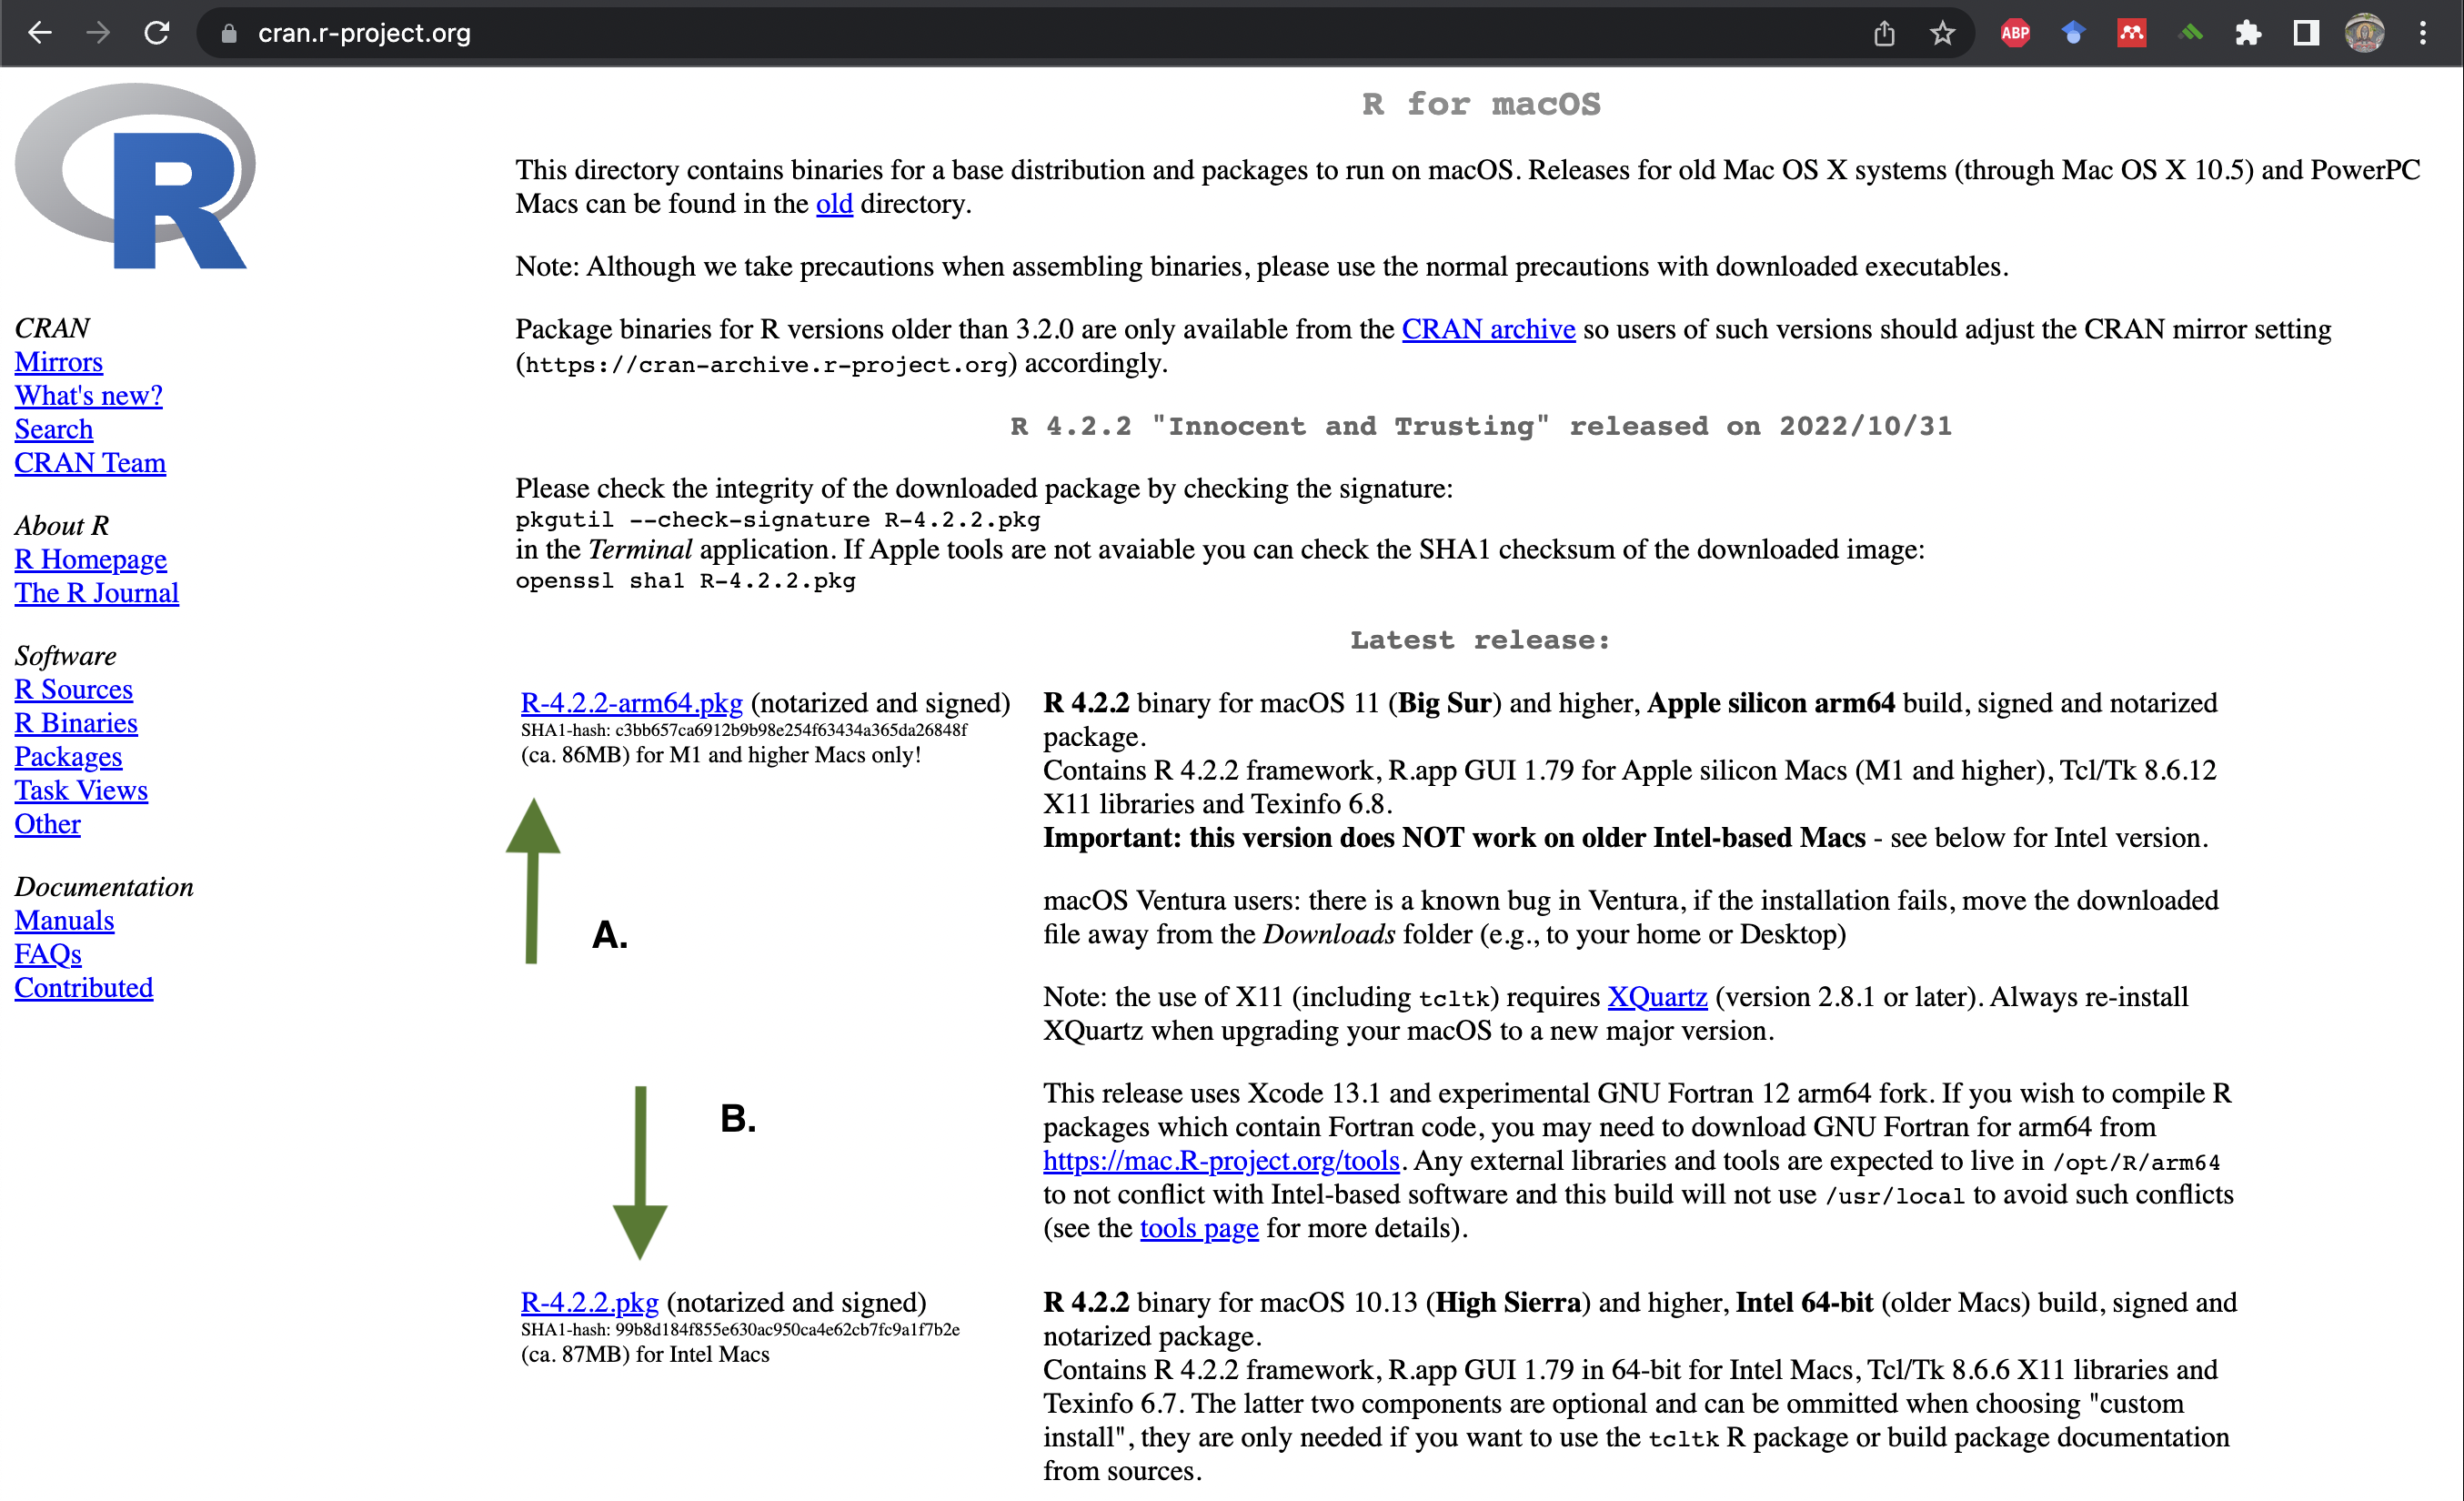
\includegraphics{images/cran_macDL} 

}

\caption{**Figure 3.** cran.R-project macOS download options}\label{fig:screenshot of macOS DL options}
\end{figure}

\hfill\break

For windows users, R will install to your ``program files'' folder. For
macOS users, you will need to move the R.app folder from the package
(once opened) and drag it into your applications folder.\\
\strut \\

\hypertarget{introduction-to-r-syntax-objects-and-functions}{%
\paragraph{Introduction to R Syntax, Objects, and
Functions}\label{introduction-to-r-syntax-objects-and-functions}}

\textbf{Second}, let's open up R to make sure that it works and to look
at some important features that will help you later on. When you open R,
you only get a text window called the console. This is where all of the
action happens and as soon as you open R, you're given some basic, but
important information.

\begin{figure}

{\centering 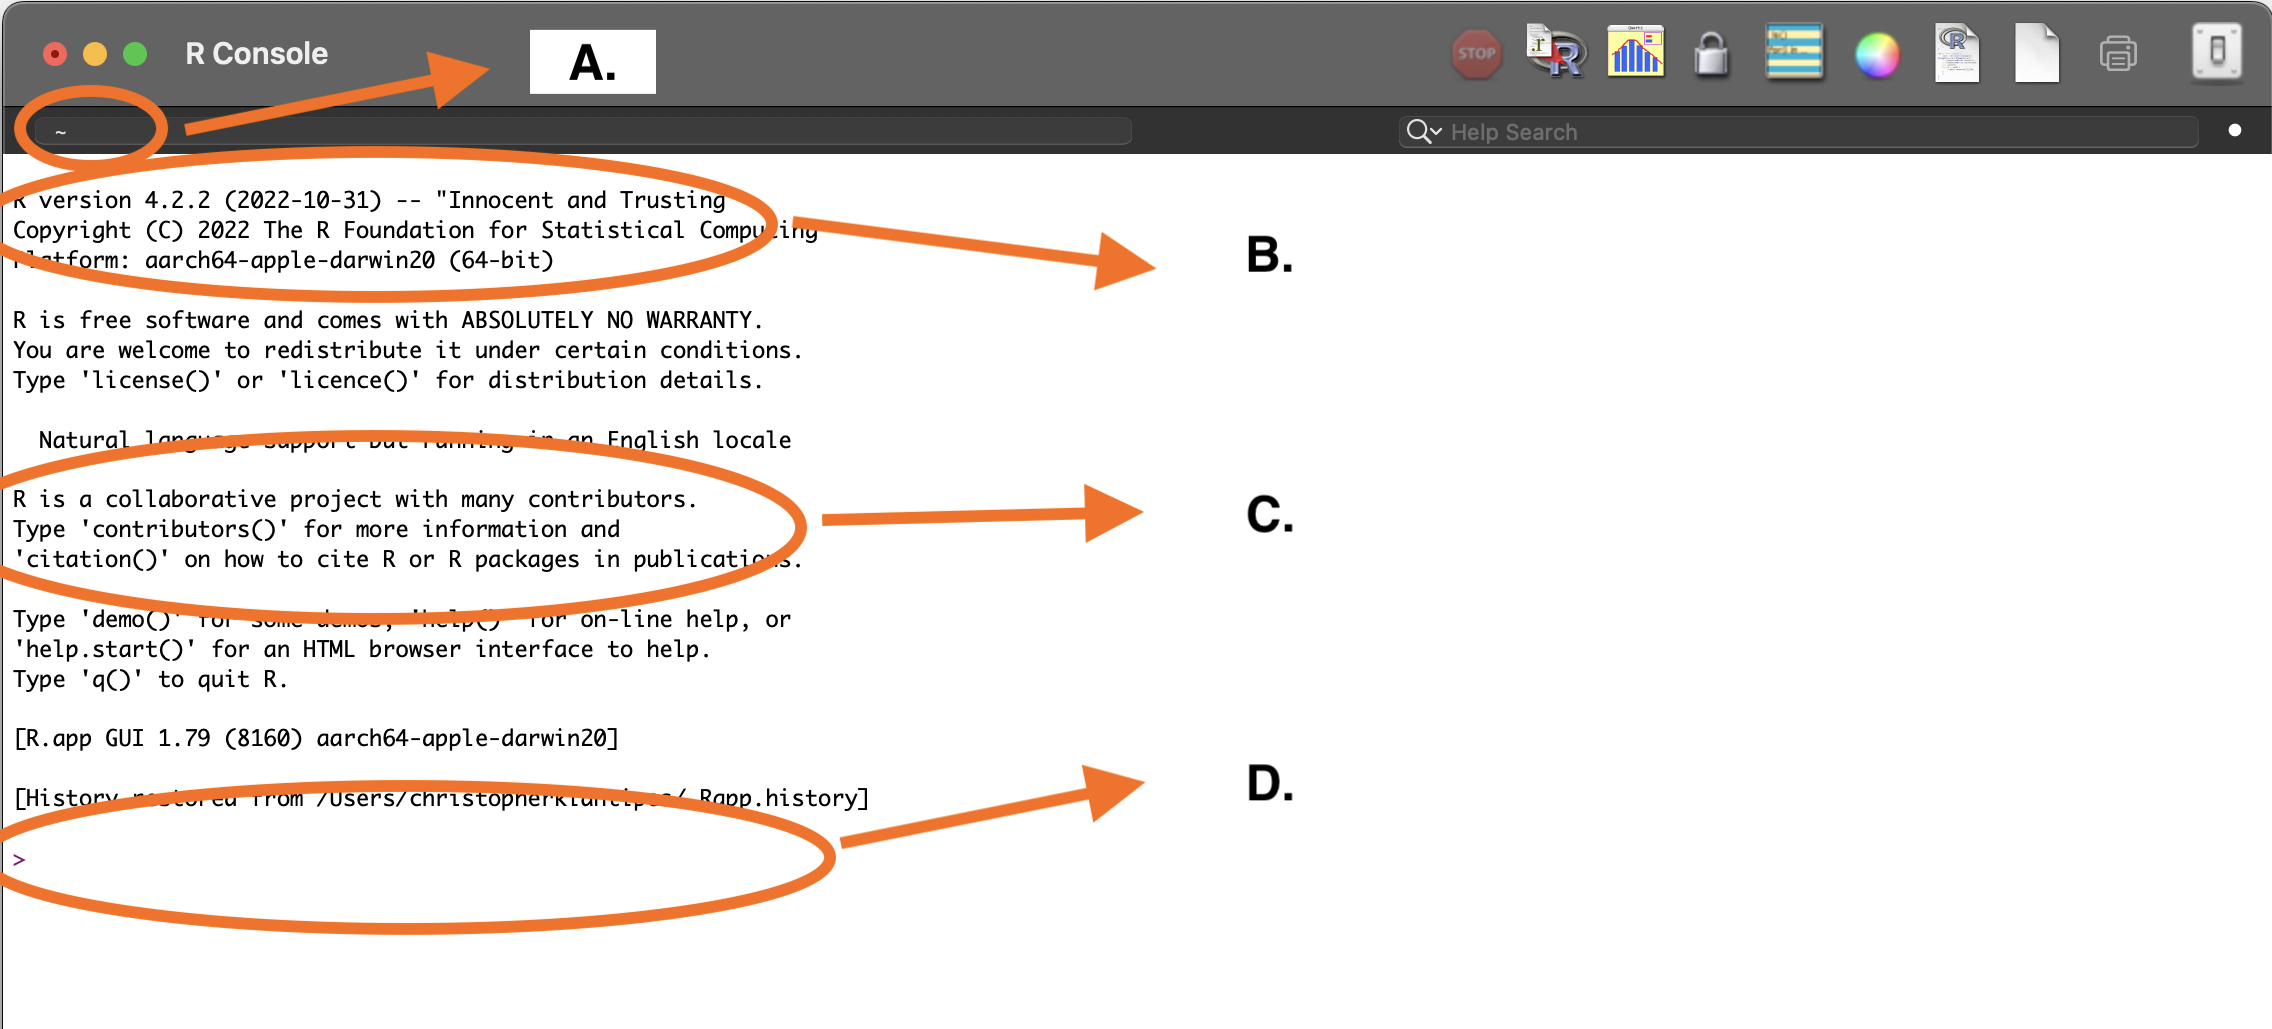
\includegraphics{images/R_console} 

}

\caption{**Figure 4.** R Console with annotations for working directory, version, and citation instructions.}\label{fig:screenshot of R console running solo}
\end{figure}

\hfill\break

Note the following: -the \emph{working directory} is the folder where R
looks when it goes to find or write things. -the software version is at
the top of the initialization text, this information is important for
citations. -the intialization text includes instructions for getting
information about licensing, help, and for citing R. -the \emph{command
line} is the line starting with ``\textgreater{}'', which is where you
politely ask R to do things for you.

We can actually try out a bit of coding at this point. Type the code
below in your R console and hit ``enter''. You can also copy-paste from
this document into the console as well.

\begin{Shaded}
\begin{Highlighting}[]
\FunctionTok{citation}\NormalTok{()}
\end{Highlighting}
\end{Shaded}

\hfill\break

This can also be written as:

\begin{Shaded}
\begin{Highlighting}[]
\FunctionTok{citation}\NormalTok{(}\StringTok{"base"}\NormalTok{)}
\end{Highlighting}
\end{Shaded}

\hfill\break

Both these commands give us the same result.

\begin{verbatim}
## 
## To cite R in publications use:
## 
##   R Core Team (2022). R: A language and environment for statistical
##   computing. R Foundation for Statistical Computing, Vienna, Austria.
##   URL https://www.R-project.org/.
## 
## A BibTeX entry for LaTeX users is
## 
##   @Manual{,
##     title = {R: A Language and Environment for Statistical Computing},
##     author = {{R Core Team}},
##     organization = {R Foundation for Statistical Computing},
##     address = {Vienna, Austria},
##     year = {2022},
##     url = {https://www.R-project.org/},
##   }
## 
## We have invested a lot of time and effort in creating R, please cite it
## when using it for data analysis. See also 'citation("pkgname")' for
## citing R packages.
\end{verbatim}

\hfill\break

\textbf{Congratulations!} If this is your first time using R, then you
just ran your first \emph{function}!

Note that ``base'' gives us the same output because the R Statistical
Computing Environment comes with a lot of basic functions (hence
``base'') that it can do. Later, we will explore how we can expand R
with ``packages'' written and maintained by other users.

We have accumulated some vocabulary at this point and it is helpful to
explain these terms and how they relate to each other here. R will do
exactly what you tell it to, so it helps to know how it thinks. The R
environment runs almost entirely by creating \emph{objects} and applying
\emph{functions} to them. Like we experienced above, \emph{functions}
make things happen. In order for R to do things with an object, it has
to know that it exists.

We could use ``base'' above because the citation() is already a part of
R and knows where to find it (its always an object). Let's learn how to
create an object.

All coding languages run on \emph{syntax} (rules for combining things
for communication). Here's some key symbols in R syntax.\\
\strut \\

\begin{longtable}[]{@{}rr@{}}
\toprule()
Syntax & Action \\
\midrule()
\endhead
= & equals sign is used to assign data to objects \\
\textless- & arrow-dash is the same as equals sign, assigns data to
objects \\
\# & hashes designate non-coding regions, used to annotate code \\
\bottomrule()
\end{longtable}

You can copy-paste the entire section of code below and run it. Another
nice thing about R is that you can submit a whole list of commands at
once, as long as each of these commands and function are entered
correctly. Because my annotations are preceded by a hash ``\#'', they're
not read as commands. As for whether one should use ``='' or
``\textless-'', there are trade-offs to either choice. I use ``=''
becauese it requires typing fewer characters.

\begin{Shaded}
\begin{Highlighting}[]
\CommentTok{\# Here, we use "=" to create an object called "x" and assign it the value of 5.}

\NormalTok{x }\OtherTok{=} \DecValTok{5}

\CommentTok{\# We can also use "\textless{}{-}" to create another object called "y" and assign it the value of 6.}

\NormalTok{y }\OtherTok{\textless{}{-}} \DecValTok{6}
\end{Highlighting}
\end{Shaded}

\hfill\break

Once you run the above code, you may notice that basically nothing
happened. R happily ran your commands and creates an object named ``x''
with a value of 5 and an object ``y'' with a value of 6. You didn't tell
R to give you any output, so none is given. Type ``x'' in the command
line and then hit ``enter''. Do the same for ``y''. R should return the
values each time after you hit ``enter''. This is rudimentary, but you
are \emph{coding} now. Also, now that we've experienced what R is like,
we can gain a better appreciation for what R Studio does for us.

\hfill\break
\hfill\break

\hypertarget{installing-r-studio}{%
\paragraph{Installing R Studio}\label{installing-r-studio}}

\textbf{Third}, you will need to
\href{https://posit.co/download/rstudio-desktop/}{download R Studio} and
install it. R Studio is available as a ``free version'' and a
``professional'' version. The links here go directly to the free
version.

\href{https://posit.co/downloads/}{\includegraphics[width=0.25\textwidth,height=\textheight]{https://d33wubrfki0l68.cloudfront.net/57299a1dcd979c623325f11bf5e5ce60f3d4eb00/e4602/wp-content/uploads/2018/10/black.png}}

The webpage should detect what sort of OS you're using and suggest the
correct version of R Studio. If it does not, there are other download
options below which correspond to various OS and OS versions. You will
notice that the webpage also tells you to install R (which we've already
done), so you can skip to ``2'' and download R Studio.

\begin{figure}

{\centering 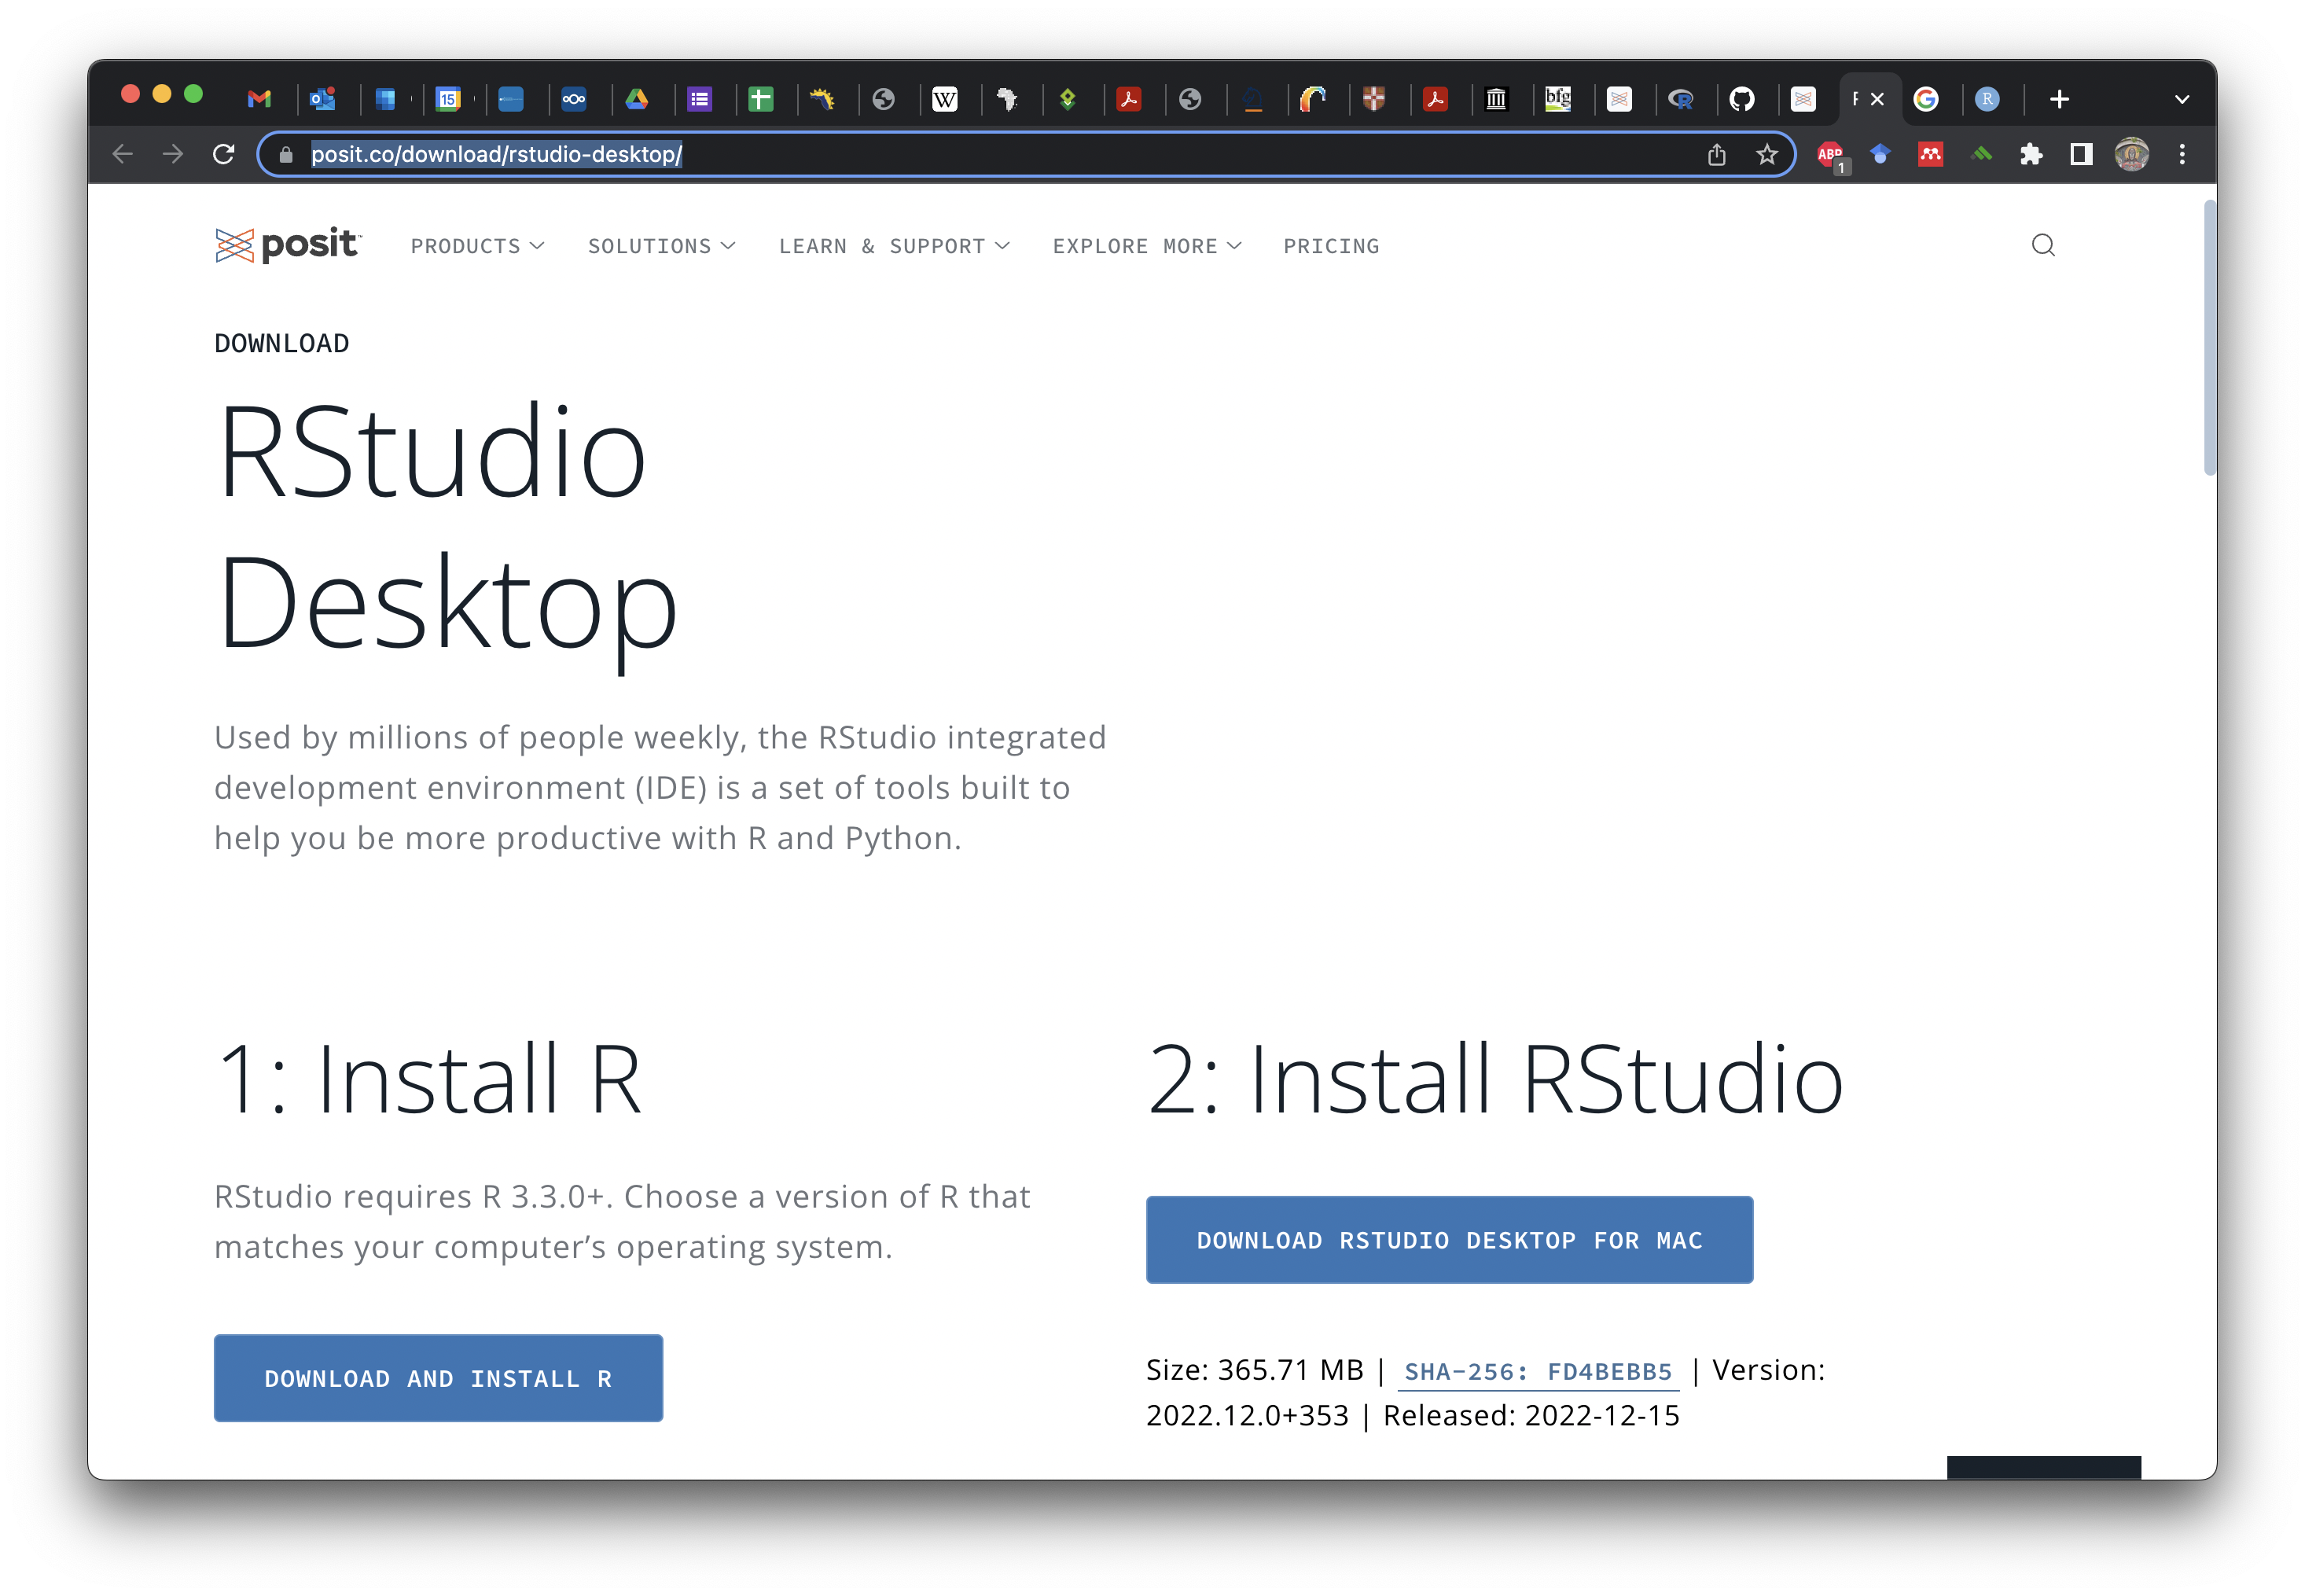
\includegraphics{images/R_studio-DL} 

}

\caption{**Figure 5.** R Studio Download Page.}\label{fig:sceenshot of R Studio Download page}
\end{figure}

\hfill\break
\hfill\break

You'll get either a .exe or a .pkg file when you download R Studio
(depending on OS) and you can then run this file and follow the prompts
from the installation wizard. Windows users will find R Studio in their
program files while masOS users will have to move the R Studio app into
the Applications folder. Make a shortcut to your desktop (Windows) or
put the app in your taskbar (macOS) for easy access.

Now, let's open R Studio and take a look at it. Double-click on the
icon.

\hfill\break
\hfill\break

You should have three panes open in the window, as shown in Fig 6.
above. The leftmost should look familiar. It is the R console! This is
where you'll enter commands to make R do things. It also shows you some
of the same information, such as the location of the working directory.
If you look carefully, this pane has two tabs: ``Console'' and ``Jobs''.
Stick with the console for now, but this area of the window is dedicated
to what R is \emph{doing}.

On the right, the top pane also has tabs: ``Environment'', ``History'',
``Connections'', ``Git'', and ``Tutorial''. We will rely on
``Environment'' and ``History'' more than the others for this tutorial.
The ``Environment'' allows us to see inside R's brain. Let's take a
quick look at how this works by entering the same commands from our
first use of base R. You can type these commands manually or copy paste
them.

\begin{Shaded}
\begin{Highlighting}[]
\NormalTok{x }\OtherTok{=} \DecValTok{5}
\NormalTok{y }\OtherTok{=} \DecValTok{6}
\end{Highlighting}
\end{Shaded}

\hfill\break

After you've run both commands (after hitting ``enter''), you should see
the environment update to include the new objects you've made. Base R
didn't show you anything, but we demonstrated that R remembered these
objects and recalled their values. Here, we can see what R knows.\\

\begin{figure}

{\centering 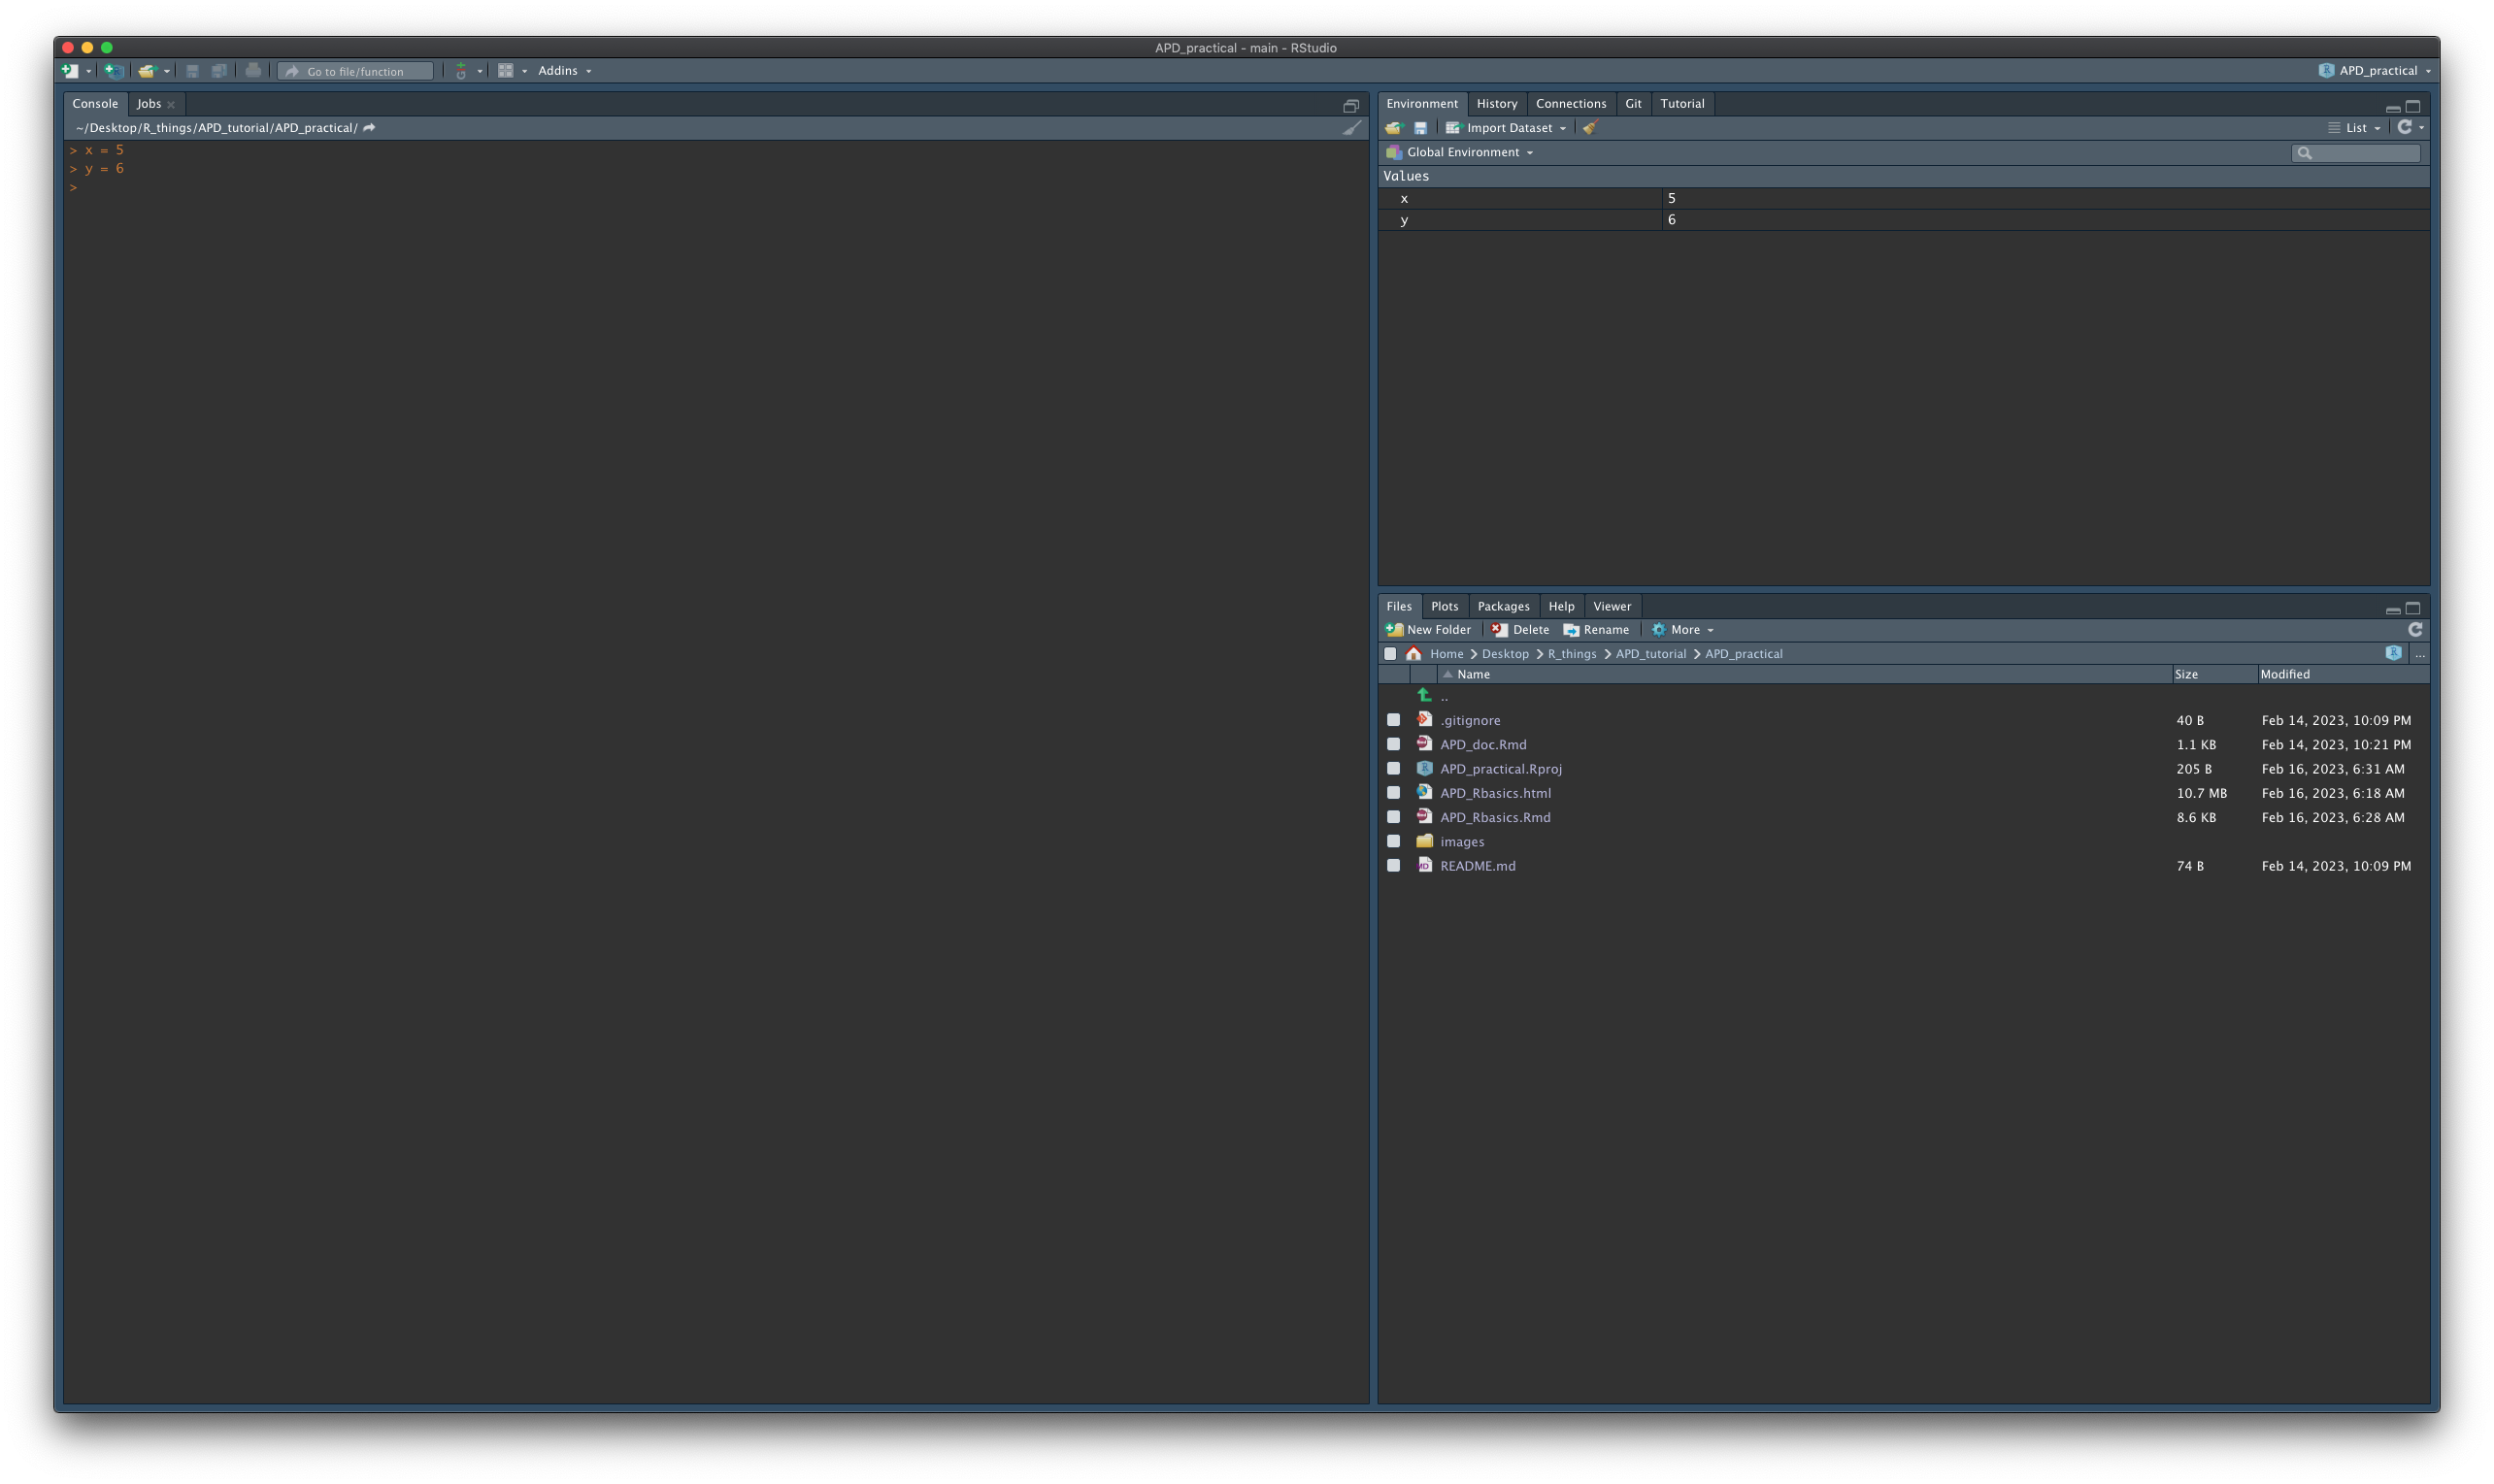
\includegraphics{images/Rst_env} 

}

\caption{**Figure 7.** R Studio showing updated Environment pane after creating objects.}\label{fig:screenshot of Rstudio step 1}
\end{figure}

\hfill\break
\hfill\break

The bottom-right pane has several file-navigation related tabs:
``Files'', ``Plots'', ``Packages'', ``Help'', and ``Viewer''. We will
make the most use of ``Files'', ``Plots'', and ``Help'' during the
workshop. It defaults to ``Files'' when we open R Studio. It will show
you the contents of the working directory as well as the file path to
the working directory (below the options - ``New Folder'', ``Delete'',
``Rename'', ``More''). This can be really helpful when troubleshooting
your code. Remember, R has to be able to find your data. In order to
help it do so, you have to know where R thinks it is. R always thinks it
is in the working directory and this pane (plus the top of the Console)
will help you figure out where R thinks that working directory is.

Another helpful pane in the bottom-right is the plots pane. R Studio
saves all of the plots that you make here. Because we've already defined
two objects, let's plot them and see what happens.

\begin{Shaded}
\begin{Highlighting}[]
\FunctionTok{plot}\NormalTok{(x, y)}
\end{Highlighting}
\end{Shaded}

\hfill\break
\hfill\break

This should create a plot in this pane, looking something like this.

\begin{figure}

{\centering 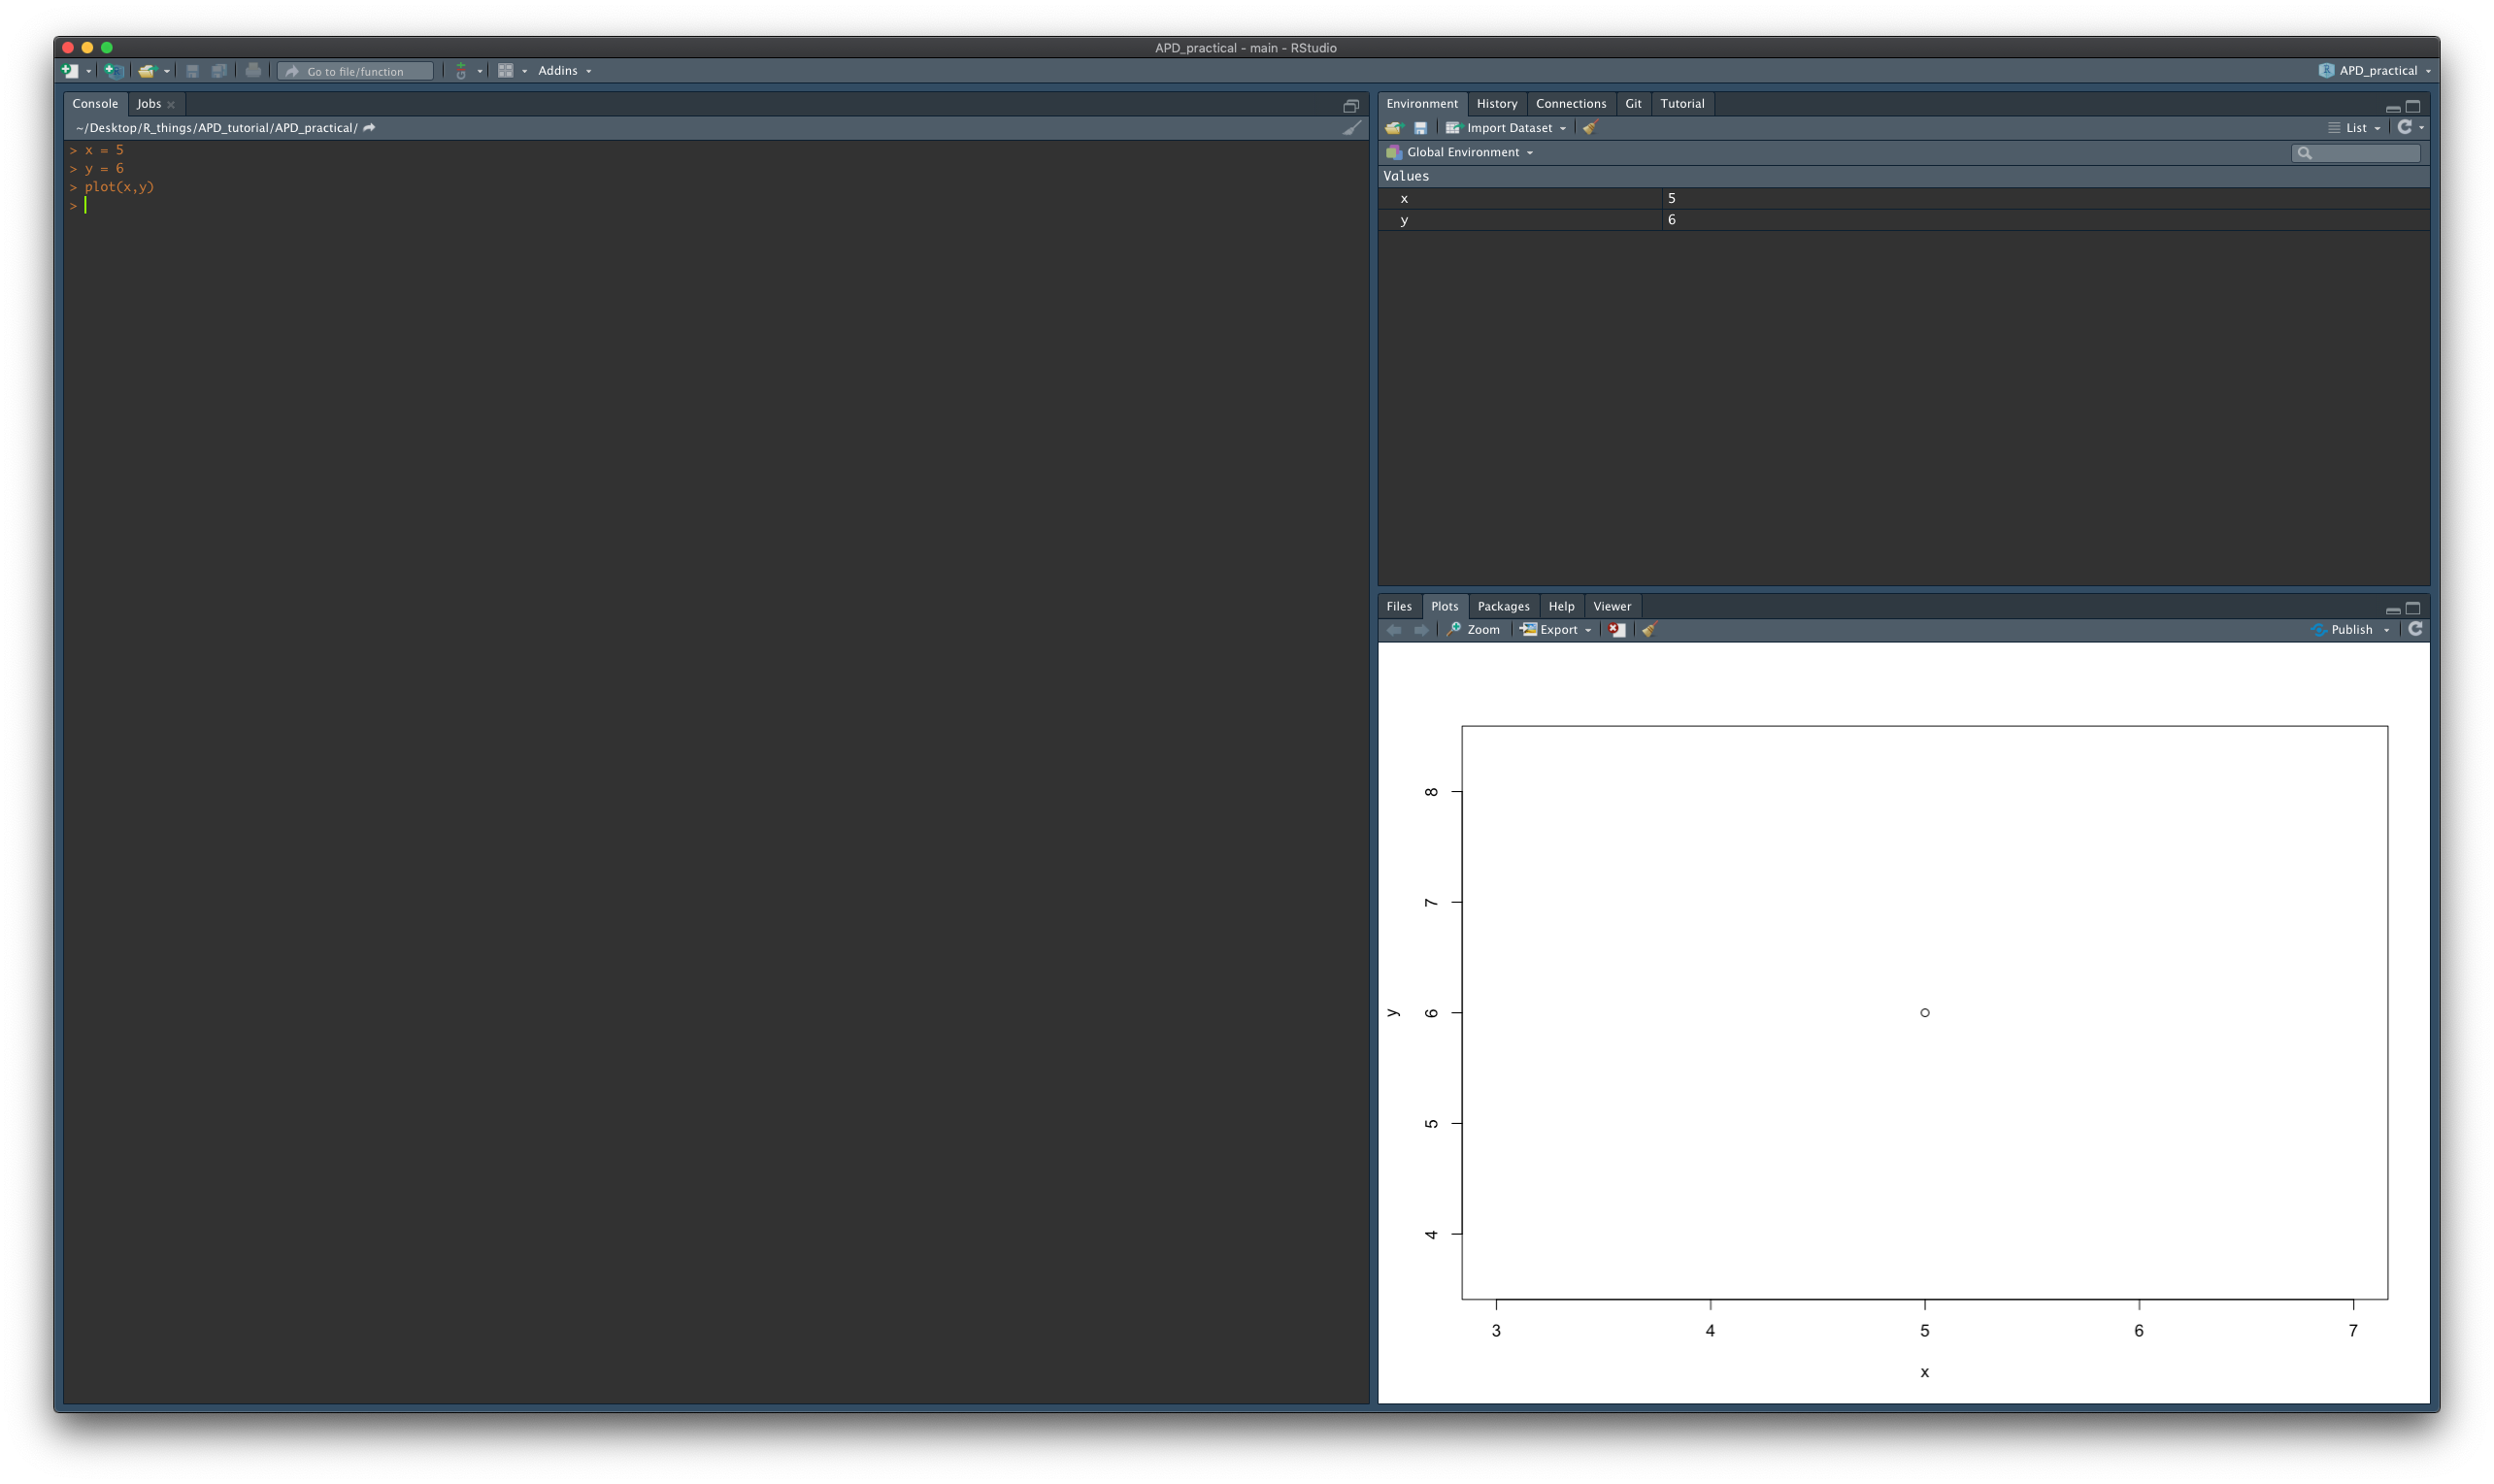
\includegraphics{images/Rst_plt} 

}

\caption{**Figure 8.** R Studio window showing plot of values of x and y.}\label{fig:plotting results screenshot}
\end{figure}

\hfill\break
\hfill\break

\textbf{Excellent!} You've already run your first function, defined
objects, and then plotted them. This is basically all that R does, but
we can create objects with multiple dimensions (vectors, matrices,
arrays!) and run complicated functions to evaluate, synthesize, and plot
this information.

\end{document}
